\documentclass[twocolumn]{article}
\usepackage{amsmath}
\usepackage{graphicx}
\usepackage{subfig}

\pagestyle{empty}
\setlength{\textwidth}{7in}
\setlength{\textheight}{9.125in}
\setlength{\columnsep}{0.3in}
\setlength{\topmargin}{-0.8in}
\setlength{\oddsidemargin}{-0.25in}
\setlength{\parindent}{5 ex}

\makeatletter
\def\@normalsize{\@setsize\normalsize{12pt}\xpt\@xpt \abovedisplayskip 11pt
plus2pt minus5pt\belowdisplayskip \abovedisplayskip \abovedisplayshortskip \z@
plus3pt\belowdisplayshortskip 6pt plus3pt
minus3pt\let\@listi\@listI}
%the following line was changed
\def\subsize{\@setsize\subsize{10pt}\xipt\@xipt}
\def\section{\@startsection{section}{1}{\z@}{24pt plus 2 pt
minus 2 pt} {12pt plus 2pt minus 2pt}{\large\bf}}
\def\subsection{\@startsection {subsection}{2}{\z@}{10pt
plus 2pt minus 2pt}{10pt plus 2pt minus 2pt}{\subsize\bf}}
\makeatother

\begin{document}
\date{}
\title{\Large\bf A Distributed Algorithm for 3D Radar Imaging}
\author{\begin{tabular}[t]{c}
Patrick S. Li, Simon Scott \\
Electrical Engineering and Computer Science\\
University of California, Berkeley
\end{tabular}}
\maketitle
\thispagestyle{empty}
\subsection*{\centering Abstract}
\vspace*{-3mm}
\textit{
eWallpaper is a smart wallpaper containing thousands of embedded, low-power processors and radio transceivers. An important application of the wallpaper is to use the radio transceivers to perform 3D radar imaging. The major obstacles in implementing the imaging algorithm on the wallpaper are the distribution of the data amongst the large number of processors, the restrictive 2D mesh topology, and the limited local memory available to each processor. Our major contribution is a distributed and memory efficient implementation of the 3D range migration algorithm that operates in realtime and achieves video framerates. A hardware simulator was built to allow rapid development and verification of eWallpaper applications. This simulator was parallelized using MPI and Pthreads, enabling fast emulation on a high-performance computing cluster. We developed a performance model and network traffic simulator to verify that our distributed algorithm will meet the framerate and memory requirements while running on the actual eWallpaper hardware.
}
\section{Introduction}

eWallpaper is a smart wallpaper with thousands of low-power, RISC-V \cite{riscv} processors embedded within the paper. These processors are connected in a 2D mesh network, spaced 25mm apart. Each processor has its own radio transceiver and antenna. One of the main objectives of eWallpaper is to use the radio transceivers to image the room. The radios attached to each of the processors transmit microwave pulses. These pulses reflect off the objects in the room and the echoes are recorded back at the transmitting antennas. The echoes are combined using an adapted version of the range migration algorithm \cite{lopez20003} to form a single three-dimensional image of the room.

\subsection{Applications of the eWallpaper Imaging System}

The ability to form 3D images of the room enables a number of useful applications, such as:
\begin{itemize}
\item gesture recognition, enabling users to control home appliances, lighting, and multimedia systems via an intuitive interface.
\item pervasive monitoring of human vital signs and automatic notification of medical personnel in case of emergencies.
\item human recognition and tracking throughout the house for security purposes. Gurbuz et al. \cite{human-recognition} describe a technique for identifying people using radar signals.
\item creation of immersive audio fields for teleconferencing \cite{immersive-audio} that track the positions of human speakers and listeners.
\end{itemize}

\subsection{Challenges with Performing Realtime Imaging}

The proposed design for eWallpaper consists of an array of $128\times128$ processors, each with an attached radio transceiver and antenna. Each processor records the responses detected at its antenna. These responses are combined to form a three-dimensional image of the room using the 3D range migration algorithm (RMA). There are three key challenges to implementing 3D RMA on eWallpaper:
\begin{enumerate}
\item The antenna responses are distributed amongst the $128\times128$ processors. Therefore, to achieve high performance, the algorithm must also be distributed.
\item In order to achieve high performance on the low-dimensional 2D mesh network, interprocessor communication requiring many network hops must be minimized.
\item The amount of local memory on each processor is extremely limited, on the order of 100KB. Furthermore, there is no global memory storage. This means that no single processor can store all the antenna responses.
\end{enumerate}

Taking these limitations into account, we developed a distributed implementation of the 3D range migration algorithm that is both memory efficient and able to achieve video framerates.

\section{The 3D Range Migration Algorithm}
\label{algorithm-section}

The algorithm presented in \cite{lopez20003} for 3D microwave imaging was adapted for implementation on eWallpaper. Here we present the underlying theory and physical model. 

During the scanning procedure, a single radio antenna will emit a continuous sinusoidal wave. The wave will reflect off the objects in the room and is received by a radio transceiver. The transmit and receive antennas are sufficiently close that they can be assumed to be colocated, as in the case of a quasi-monostatic radar. The amplitude of the received sine wave and the phase difference between the transmitted and received wave are recorded. For each antenna in turn, this procedure is repeated over a range of evenly spaced frequencies. 

In our setup, we have 128$\times$128 antennas, each of which step through 256 frequencies. Thus the input to the imaging algorithm is a 3D array of 128$\times$128$\times$256 amplitudes and phase differences.

We will assume, in the development of the algorithm, that the speed of light is known and constant for all points in the scene. We also do not consider any refraction or attenuation effects. We will model the scene as a collection of discrete point targets distributed uniformly throughout the imaged region. Each point target, at position $(x,y,z)$, is fully described by a single real number, $0 \leq r \leq 1$, which represents its reflectivity. A unit-amplitude sine wave emitted by a radio antenna is assumed to travel, unimpeded, to all points in the scene. It reflects off the targets and arrives back at the radio transceiver with amplitude $r$. The superposition of the reflected waves from each target is recorded by the radio transceiver. This physical model is minimal but is sufficient for the purposes of imaging.

\begin{figure}[!h]
\centering
\includegraphics*[width=0.3\textwidth]{figures/antenna.pdf}
\caption{Geometric layout of antenna plane and a single point target}
\label{antenna}
\end{figure}

Formally, consider a single antenna at position $(x', y', 0)$. Let $d = \sqrt{(x'-x)^2+(y'-y)^2+z^2}$ be the distance from the antenna to a target at position $(x,y,z)$ (Figure \ref{antenna}). The time taken for the sine wave, emitted by the antenna, to travel to the target and back again is $t = \frac{2d}{c}$, where $c$ is the speed of light. In that time, the phase of the transmitted sine wave has advanced by $\phi = \omega t$, where $\omega$ is the angular frequency. The amplitude of the sine wave received by the transceiver and the phase difference between the transmitted and received sine waves can be represented as a single complex number, $r e^{-j \phi}$, where the amplitude of the wave is represented by the magnitude, and the phase difference is represented by the angle. Thus, the final received signal at the transceiver, which is the superposition of the reflected waves from each point target, is given by
%
\begin{gather}
s(x', y', z=0, \omega) = \int \int \int r(x,y,z) e^{-j \phi(x,y,z)} dx dy dz \nonumber \\
= \int \int \int r(x,y,z) e^{-j \frac{2\omega}{c} \sqrt{(x'-x)^2 + (y'-y)^2 + z^2}} dx dy dz.
\end{gather}

The received signal has, thus far, been described as the superposition of the reflections from each point target. Alternatively, we can equivalently interpret the point targets to be, themselves, emitting sine waves which travel at half the speed of light, $\frac{c}{2}$, towards the transceiver. Under this interpretation, the scene generates a wavefield, $s(x,y,z,\omega)$, and the transceivers sample the wavefield on the plane $z=0$ to obtain $s(x,y,z=0,\omega)$. Our goal is to recover the full wavefield, $s(x,y,z,\omega)$ given only $s(x,y,z=0,\omega)$.

The wavefield at depth $z$ can be recovered by back propagating the recorded wavefield, $s(x, y, z=0, \omega)$, from the antenna to the target. This can be achieved by simply swapping the sign of the phase delay term, thus representing propagation backwards in time, and summing over the contribution from each antenna.
%
\begin{gather}
s(x,y,z,\omega) =\int\int s(x',y',z=0,\omega) \cdot \nonumber \\
e^{j \omega \frac{2}{c} \sqrt{(x'-x)^{2}+(y'-y)^{2}+z^{2}}} dx'dy'
\end{gather}
%
After back propagation, the final 3D image can be reconstructed by integrating the wavefield over all frequencies.
\begin{equation}
s(x,y,z)=\int s(x,y,z,\omega) d\omega
\end{equation}

While the above algorithm is intuitive, integrating over all frequencies and antenna positions, for each point in the scene, makes computation prohibitively expensive. For 128$\times$128 antennas and 256 frequencies, it took over two and a half hours on a 24 core cluster to image a room. To make computation tractable, we pre-transform our received signal to the frequency domain, where we will do all our computations, and then transform back to the spatial domain.

Let $S(k_x,k_y,z=0,\omega) = \text{FT}_{x,y} \{ s(x, y, z=0, \omega) \}$ be the Fourier transform of the recorded wavefield with respect to $x$ and $y$. Back propagation becomes an efficient element-wise multiplication in the spatial frequency domain.
\begin{equation}
	S(k_x, k_y, z, \omega) = S(k_x, k_y, z=0, \omega) e^{j k_z z},
\end{equation}
where
\begin{equation}
  	k_z = \sqrt{ (\frac{2 \omega}{c}) ^ 2 - k_x^2 - k_y^2}.
\end{equation}

The image in the frequency domain is reconstructed, as before, by integrating the back propagated field over all frequencies.
\begin{equation}
	S(k_x, k_y, z) = \int S(k_x, k_y, z=0, \omega) e^{j k_z z} d\omega. \label{eq:stolt-integral}
\end{equation}
Finally, we use the inverse Fourier transform to recover the image in the spatial domain, $s(x,y,z) = \text{IFT}_{k_x, k_y} \{ S(k_x, k_y, z) \}$. 

The pre and post Fourier transforms can be done efficiently using FFTs, and back propagation is a fast element-wise multiplication in the frequency domain. The only remaining integral at this point is given by equation \ref{eq:stolt-integral}, which as a further optimization, can be computed efficiently by noting that it has a similar form to the inverse Fourier transform. 

By resampling $S(k_x, k_y, z=0, \omega)$ at evenly spaced intervals of $k_z$ (a technique known as Stolt interpolation in the seismic imaging field),
\begin{equation}
	S'(k_x, k_y, z=0, k_z) = \text{Stolt}\{ S(k_x, k_y, z=0, \omega) \},
\end{equation}
the integral in equation \ref{eq:stolt-integral} can be efficiently computed using an inverse FFT. Resampling may be done using linear interpolation.
\begin{gather}
	S(k_x, k_y, z) = \int S(k_x, k_y, z=0, \omega) e^{j k_z z} d\omega 	\nonumber \\
	= \int S'(k_x, k_y, z=0, k_z) e^{j k_z z} dk_z	\nonumber \\
	= \text{IFT}_{k_z} \{ S'(k_x, k_y, z=0, k_z) e^{j k_z z_0} \},
\end{gather}
where $z_0$ is the minimum distance from the antenna plane that we wish to image.

The whole algorithm is then given as follows: \\
1. Pre-transform the received signal to the spatial frequency domain using a 2D FFT.
\begin{equation}
	S(k_x,k_y,z=0,\omega) = \text{FT}_{x,y} \{ s(x, y, z=0, \omega) \}
\end{equation}
2. Perform Stolt interpolation and back propagation in the spatial frequency domain.
\begin{gather}
	S(k_x, k_y, z) = 	\nonumber \\
	\text{IFT}_{k_z} \{ \text{Stolt}\{ S(k_x, k_y, z=0, \omega) \} e^{j k_z z_0} \}
\end{gather}
3. Transform the reconstructed image back to the spatial domain using a 2D IFFT.
\begin{equation}
	s(x, y, z) = \text{IFT}_{k_x, k_y} \{ S(k_x, k_y, z) \}
\end{equation}
The reconstructed image, $s(x,y,z)$, is a 3D array whose values represent the reflectivity at each point the room.

\section{Implementation on a 2D Mesh Network}
\label{algorithm-implementation}

A single sheet of eWallpaper contains 16384 low-power Rocket processors, arranged in a $128\times128$ array. The interprocessor network on eWallpaper is formed from a single layer of printed wires, and thus is restricted to low-dimensional topologies. Thus, bi-directional links connect each eWallpaper processor to only its four immediate neighbors resulting in a 2D mesh network.

The Rocket processor is a 6-stage, in-order processor, based on the RISC-V \cite{riscv} ISA, with a clock speed of 1GHz. It has a 64KB L1 cache, 100KB of on-chip main memory, and a floating-point unit capable of approximately 200 MFlops/s. There is no additional off-processor memory in eWallpaper.

The implementation of the imaging algorithm described in Section~\ref{algorithm-section} on eWallpaper relies upon two fundamental operations: the row-wise transpose and the column-wise transpose.

\subsection{The Row-wise Transpose}

Assuming there are N processors in each row of the mesh network, with each processor containing M data values, the values stored on processor $n \in \{1 \ldots N\}$ can be expressed as:
\[ D_n = \{d_{n1}, d_{n2}, d_{n3}, ..., d_{nM}\}. \]
After performing the row-wise transpose, the values stored on processor $n$ are:
\[ D_n = \{d_{1n}, d_{2n}, d_{3n}, ..., d_{Mn}\}. \]
Therefore, after the transpose, the $n^{th}$ processor in the row contains the $n^{th}$ value stored by each processor before the transpose.

Figure~\ref{row_wise_transpose} shows an example of a row-wise transpose on a $3\times3$ processor array. The array before the transpose is shown on the left of the figure, with each processor storing the antenna responses for 3 frequencies (represented by 3 circles at each processor). In order to perform the row-wise transpose, every processor first sends its locally stored data to its left and right neighbors. Once its own data has been sent, each processor waits to receive the complete packet from its left neighbor. The processor extracts the required value from this packet and forwards the packet onto its right neighbor. Processor $n$ will extract the $n^{th}$ value from the packet. Similarly, the processor will receive a packet from its right neighbor, extract the required value, and forward the packet onto its left neighbor. In this way, a full row-wise transpose can be performed in $N-1$ hops for a row of $N$ processors.

\begin{figure}[!h]
\centering
\includegraphics*[width=0.5\textwidth, viewport = 10 10 620 150]{figures/row_wise_transpose.pdf}
\caption{A 3x3 processor array, before (left) and after (right) the row-wise transpose}
\label{row_wise_transpose}
\end{figure}

The array on the right of Figure~\ref{row_wise_transpose} shows the data stored in each processor after the transpose. The processors in the first column store the first frequency values, the processors in the second column store the second frequency values, etc. Note that during the row-wise transpose operation, interprocessor communication occurs only between processors in the same row. This allows all rows to be transposed at the same time.

This is similar to the Ring Exchange Algorithm described by Christara et al. \cite{efficient-transposition} for ring networks. Christara et al. argue that store and forward is better than wormhole routing for the transposition operation on a ring network, as each processor requires data from all other processors. Furthermore, they prove that this approach is optimal for ring networks, as it performs the transpose in $N-1$ hops, where $N$ is the number of nodes.

Note that in our row-wise transpose, each processor forwards the entire original packet after extracting the required values. In the Ring Exchange Algorithm, each processor \emph{removes} the values it requires from the packet before forwarding. The result is that our approach incurs twice the total bandwidth cost as the Ring Exchange Algorithm.

\subsection{The Column-wise Transpose}

The column-wise transpose, shown in Figure~\ref{column_wise_transpose}, operates in a similar fashion to the row-wise transpose, except that each processor communicates with the other processors in the same column, instead of the same row.

\begin{figure}[!h]
\centering
\includegraphics*[width=0.5\textwidth, viewport = 40 10 650 150]{figures/column_wise_transpose.pdf}
\caption{A 3x3 processor array, before and after the column-wise transpose}
\label{column_wise_transpose}
\end{figure}

\subsection{The Distributed 3D Imaging Algorithm}

With the row-wise and column-wise transpose operations defined, the imaging algorithm described in Section~\ref{algorithm-section} can be expressed as a sequence of computation and communication steps, as shown in Figure~\ref{algorithm_labeled}. These operations run on each processor in the network. The yellow boxes in the diagram represent computational operations, while the grey boxes represent communication.

\begin{figure}[!h]
\centering
\includegraphics*[width=0.3\textwidth, viewport=10 70 430 750]{figures/algorithm_labeled.pdf}
\caption{The distributed 3D range migration algorithm that runs on each processor}
\label{algorithm_labeled}
\end{figure}

At the start of the algorithm, each processor contains the responses recorded at its own antenna, for each of the 256 frequency steps. The 2D FFT across the entire dataset, with respect to $x$ and $y$, is computed as a set of 1D FFTs along the $x$-axis, followed by a set of 1D FFTs along the $y$-axis. The first step in the 2D FFT is a row-wise transpose, resulting in each processor storing the responses at all 128 $x$ positions for two frequencies. The processor then performs two 128-point 1D FFTs on the locally stored data. This is followed by a column-wise transpose, resulting in each processor now containing the responses at all 128 $y$ positions, for a particular $k_x$ value and two frequencies. Finally, each processor once again performs two 128-point 1D FFTs on locally stored data, completing the 2D FFT.

After the 2D FFT, a row-wise transpose is performed, placing all 256 frequency values for a particular $k_x$ and $k_y$ at each processor. The processor is now able to perform back propagation and Stolt interpolation on locally stored data, without further communication. Back propagation involves multiplying each stored value by a unique complex number. Stolt interpolation is achieved using linear interpolation. Both the back propagation coefficients and the linear interpolation indices are precomputed to accelerate computation.

The final 3D inverse FFT is implemented using three separate 1D inverse FFTs, with interleaving row and column transposes. At the end of the algorithm, each processor contains the reflectivity at all 256 depths, $z$, at a particular $(x,y)$ position.

\section{High Performance Functional Simulator}

To aid the development of the imaging algorithm, we created a functional simulator for fast prototyping and debugging of eWallpaper applications. eWallpaper applications are written in Single Program Multiple Data (SPMD) style, and one program instance is launched per simulated processor. Each simulated processor knows its own coordinates on the eWallpaper processor grid, and has access to a minimal set of communication functions for sending and receiving data packets from its immediate neighbors. In order to achieve fast emulation of a large number of processors, the simulator was parallelized to run on an MPI cluster. Within an MPI node, multiple virtual processors are simulated using Pthreads (see Figure \ref{mpi_sim}).

\begin{figure}[!h]
\centering
\includegraphics*[width=0.3\textwidth]{figures/mpi_sim.pdf}
\caption{Structural overview of MPI-based functional simulator}
\label{mpi_sim}
\end{figure}

The following basic functions are provided for interprocessor communication:
\begin{itemize}
	\item \textbf{send\_message(direction, message, message\_size)} sends a message, of the specified message size, to one of the four neighboring processors.
	\item \textbf{receive\_message(direction)} receives a message from one of the four neighboring processors. A pointer to the start of the message buffer is returned.
	\item \textbf{set\_receive\_buffer(direction, buffer)} instructs the network router to place incoming packets in the provided buffer.
\end{itemize}

{\em send\_message} blocks until the network router is free to send and the receiving processor has space available to hold the message. Note that {\em send\_message} returns as soon as message transmission begins, {\em not} when message transmission is completed. {\em receive\_message} blocks until there is a complete message waiting in the network buffer. 

Network functions for communication between virtual processors on the same MPI node are implemented using shared memory and mutexes. Across MPI node boundaries, eWallpaper network functions are implemented on top of MPI \emph{Isend} and \emph{Irecv} operations. These MPI node boundaries are invisible to the eWallpaper application.

For computationally intensive applications, the simulator can be configured to run on more MPI nodes, with a smaller number of virtual processors per node. For faster prototyping and debugging, we can configure the simulator to emulate {\em all} the virtual processors on a single node. This allows the entire simulation to be run on a single laptop, hence avoiding the lengthy job-queue system on NERSC and enabling a shorter edit-test-debug cycle.

\section{Simulated Imaging Results}

Our distributed algorithm was tested on the functional simulator running on a 64 core cluster. Antenna responses were artificially generated for three different input scenes. Figure \ref{3_points_input} shows an input scene consisting of three points of varying reflectivities. The top-left point is the least reflective and the bottom-right point is the most reflective. Figure \ref{3_points_output} shows the scene that our algorithm reconstructed. The brightest object in the recovered image corresponds to the point with highest reflectivity. 

\begin{figure}
\begin{centering}

\subfloat[Input Scene]{
	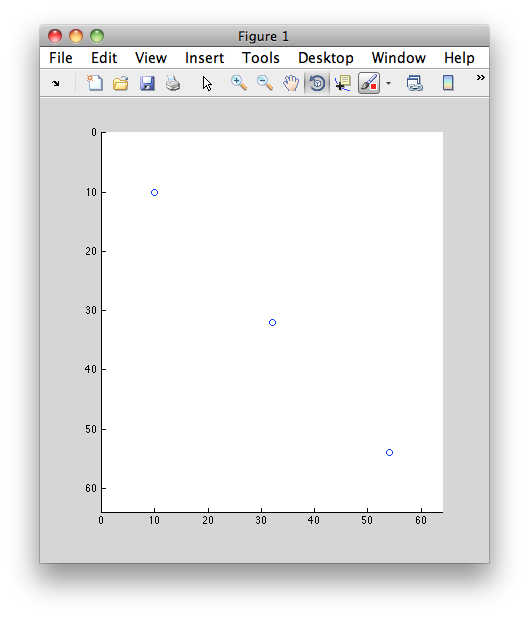
\includegraphics[bb=80bp 80bp 460bp 500bp,clip,height=4cm]{figures/3_points_input.png}
	\label{3_points_input}}
\subfloat[Reconstructed Scene]{
	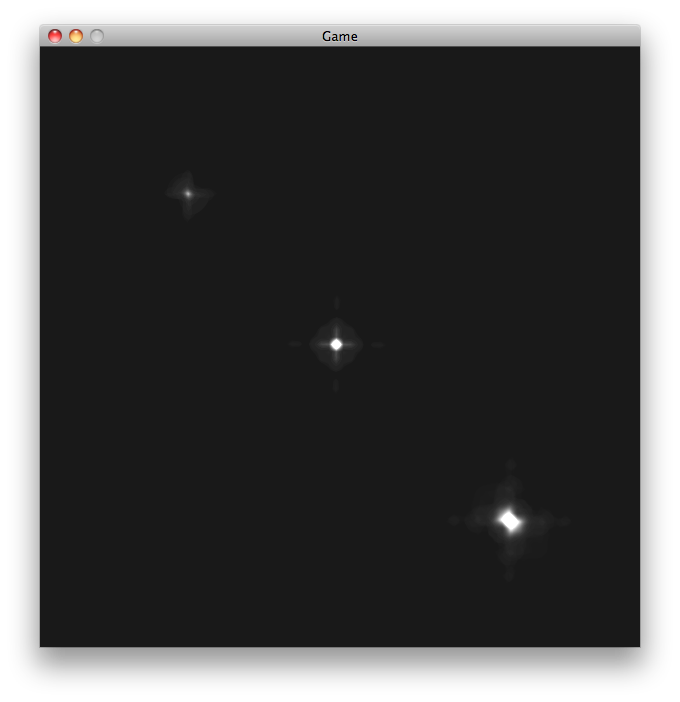
\includegraphics[bb=100bp 100bp 600bp 600bp,clip,height=4cm]{figures/3_points.png}
	\label{3_points_output}}
	
\end{centering}
\caption{Scene with three points of different reflectivities}
\end{figure}

Figure \ref{sphere_input} shows an input scene consisting of a collection of points distributed along the surface of a sphere. Figure \ref{sphere_output} shows that the sphere is correctly reconstructed by our algorithm. For Figure \ref{skull_angle1} and \ref{skull_angle2}, the antenna responses are artificially generated from a set of points taken from the Stanford volume data archive \cite{levoy1988display}, which was obtained from a CT scan of a human head. The recovered 3D image of the head is shown from two different angles.

\begin{figure}
\begin{centering}

\subfloat[Input Scene]{
	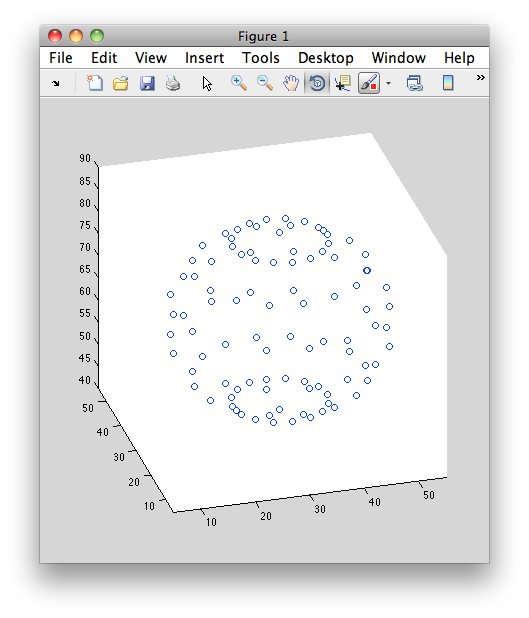
\includegraphics[bb=70bp 80bp 460bp 500bp,clip,height=4cm]{figures/sphere_input.png}
	\label{sphere_input}}
\subfloat[Reconstructed Scene]{
	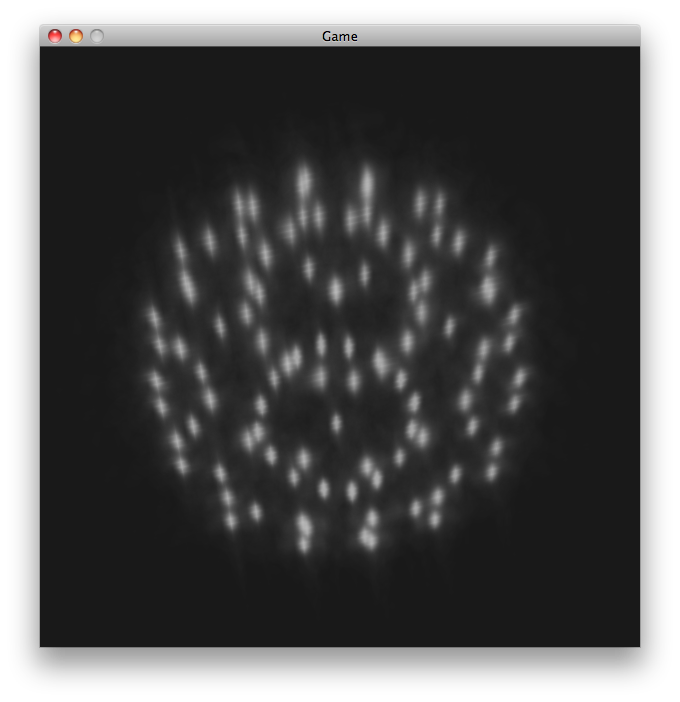
\includegraphics[bb=100bp 100bp 600bp 600bp,clip,height=4cm]{figures/sphere.png}
	\label{sphere_output}}
	
\end{centering}
\caption{Scene with points distributed along a spherical surface}
\end{figure}


\begin{figure}
\begin{centering}

\subfloat[Reconstructed Scene]{
	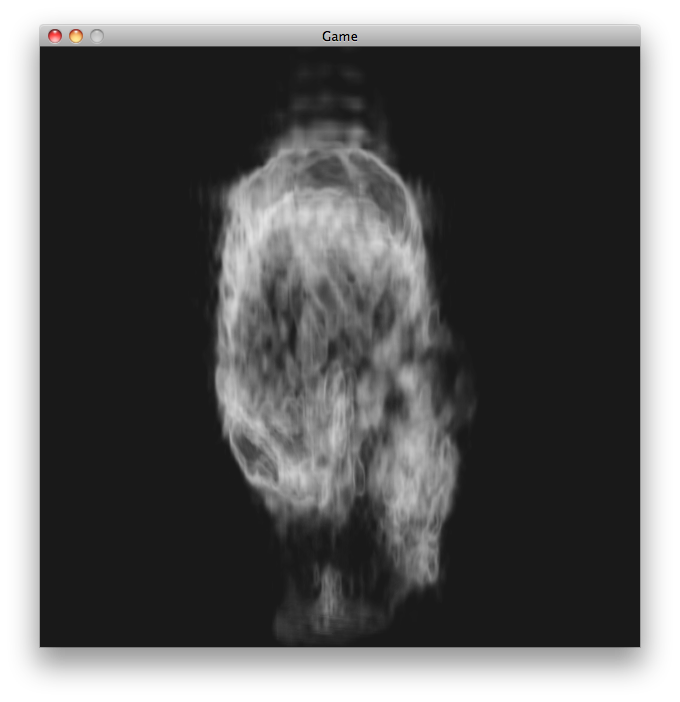
\includegraphics[bb=110bp 70bp 600bp 600bp,clip,height=4cm]{figures/skull4.png}
	\label{skull_angle1}}
\subfloat[Reconstructed Scene]{
	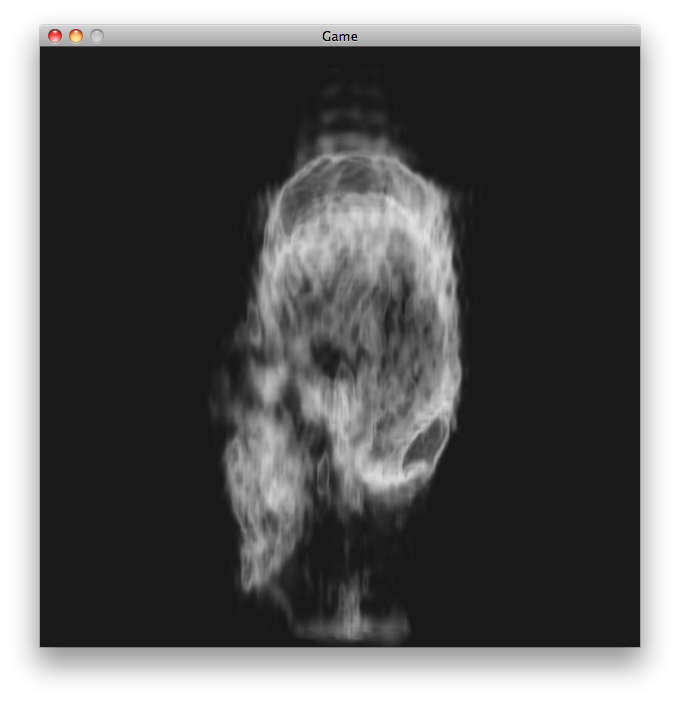
\includegraphics[bb=100bp 70bp 600bp 600bp,clip,height=4cm]{figures/skull6.png}
	\label{skull_angle2}}
	
\end{centering}
\caption{Two angles of the reconstructed scene from a CT scan}
\end{figure}

\section{Investigation of Design Parameters}


While the functional simulator allowed us to verify the correctness of our distributed algorithm, it gave no measure of the projected performance of the algorithm on eWallpaper. To predict the performance, we developed a timing model of the application code running on the functional simulator. This model, which is described below, shows that the code spends more than 90\% of its time communicating. A network simulator was therefore also developed to aid investigation into the effects of different communication patterns and network parameters on performance.
 
\subsection{Timing Model}

We assume that there are $N_{ant}\times N_{ant}$ antennas arranged in a square array, and that each antenna steps through $N_f$ frequencies.

 Let $B$ be the network bandwidth, $L$, the network latency from one processor to a neighbor, $T_M$, the time to load or store a complex floating point number, and $T_F$, the time to perform a floating-point arithmetic operation. Table~\ref{timing-model-table} shows the time taken by each of the main steps in the distributed imaging algorithm described in Section~\ref{algorithm-implementation}.

\begin{table}[!h]
\centering
\caption{Time for Individual Operations}
\begin{tabular}{l p{4.5cm}}
\hline
\bf Operation & \bf Time \\
\hline
send\_left\_right & $N_f \times T_M + 4L$ \\
receive\_and\_forward & $ \left( N_{ant} - 1 \right) \times \left( \frac{N_f \times 8}{B} + L \right)$ \\
fft & $ N_f \times \log_2N_f \times (8T_F + 3T_M) $ \\
ptwise\_vector\_mult & $ N_f \times (6T_F + 3T_M) $\\
stolt\_interpolation & $ N_f \times \left(10T_F + 4T_M \right) $ \\
\hline
\end{tabular}
\label{timing-model-table}
\end{table}

By combining the times for individual operations with the complete algorithm, as depicted in Figure~\ref{algorithm_labeled}, the time to compute a complete image can be expressed as:
{\small
\[
\begin{array}{l l l}

T & = & 6 \times (\text{send\_left\_right} + \text{receive\_and\_forward}) + \\
 &   & 5 \times \text{fft} + \text{ptwise\_vector\_mult} + \text{stolt\_interpolation} \\ 
 & = & N_f \big( T_F(16 + 40\log_2N_f) + T_M(15\log_2N_f + 13) \big) + \\
 &   & 6 \left( N_{ant} - 1 \right) \left( \frac{8N_f}{B} + L\right) + 24L

\end{array}
\]
}
\normalsize

\subsection{Network Simulator}

A discrete-event simulator was developed to help analyze the effect of interprocessor communication on algorithm performance. The simulator maintains an event queue for each processor in the network. Whenever communication occurs between two neighboring processors, one or more of the following events are enqueued at both processors:
\begin{enumerate}
\item Transmission of the packet head at the sender
\item Transmission of the packet tail at the sender
\item Reception of the packet head at the receiver
\item Reception of the packet tail at the receiver
\item Transmission and reception of acknowledgement messages
\item Buffer overflows and underflows
\end{enumerate}
To accurately predict the performance of the algorithm on the actual eWallpaper hardware, the expected wallpaper bandwidth and latency parameters were used in modeling the events. 

Using the network simulator, we can determine the effect that bandwidth, latency, and antenna array size have on framerate, CPU utilization, and memory usage. The network simulator was also used to investigate the performance of different communication patterns, as shown in Figure~\ref{comm_patterns_arrows}. In this diagram, the arrows indicate the migration of data to the processors that are actively involved in the computation (the red-shaded blocks).

\begin{figure}[!h]
\centering
\includegraphics*[width=0.4\textwidth, viewport=80 10 700 590]{figures/comm_patterns_arrows.pdf}
\caption{Possible communication patterns for the imaging algorithm}
\label{comm_patterns_arrows}
\end{figure}

The single-node pattern is the simplest. All processors forward their local data to a single node, which then processes all the data sequentially. Once all the data is on the processing node, no more communication occurs, and all other processors are idle. 

Under the single-column pattern, each processor sends its data left until it reaches the left-most processor in its row. All computation is then done by the processors in the first column. These processors only need to communicate with each other when performing a column-wise transpose. Row-wise transposes can be done without communication.

In the cluster pattern, all data is sent to a small cluster of processors in the center of the array. All the computation is then performed by this cluster. Since the cluster is small, row-wise and column-wise transposes can be performed with fewer network hops.

The fully-distributed pattern represents communication for the algorithm described in Section \ref{algorithm-implementation}. All data and computation is evenly distributed amongst the processors. The row-wise and column-wise transpose operations involve all the processors in the row or column.

\section{Performance Results}

The time taken to reconstruct a single frame for each communication pattern, as determined by the network simulator, is shown in Figure \ref{time vs comm pattern}. The lower half of each bar (shown in blue) represents the time that each processor spends communicating with its neighbors, while the upper half (shown in red) represents the average time spent computing. The fully distributed pattern is the fastest, requiring just 13 milliseconds per frame. The only other pattern able to deliver video framerates is the $16\times16$ cluster. 

The graph highlights the communication versus computation tradeoff inherent to each communication pattern. 
The communication patterns that have large numbers of processors actively involved in the computation are dominated by communication time, such as the Fully Distributed pattern, which spends 96\% of its time communicating.
In contrast, the communication patterns with small numbers of processors are dominated by computation time, such as the Single Node pattern, which spends 97\% of its time computing.

\begin{figure}[!h]
\centering
\includegraphics*[width=0.4\textwidth]{figures/chart5.pdf}
\caption{Time vs. communication pattern}
\label{time vs comm pattern}
\end{figure}

Figure \ref{mem vs comm pattern} shows the peak required memory per node for the different communication patterns. The larger the number of active processors in the pattern, the less the required memory per active node. Since each processor has only 100KB of local memory available, the only viable patterns are the Fully Distributed and 16x16 Cluster. 

Since the fully distributed pattern is the fastest and requires the least memory, it shall be selected as the pattern of choice for our distributed range migration algorithm. All further analysis therefore assumes the use of this pattern.

\begin{figure}[!h]
\centering
\includegraphics*[width=0.4\textwidth]{figures/chart6.pdf}
\caption{Memory vs. communication pattern}
\label{mem vs comm pattern}
\end{figure}

Figure \ref{framerate vs resolution} shows that as we increase the width of the antenna array, and hence distribute the data amongst more processors, the framerate decreases due to the increased communication. Note that in all the experiments  we constrain the number of frequencies to be twice the antenna array width. At our planned resolution of 128 antennas $\times$ 128 antennas $\times$ 256 frequencies, we achieve 75 frames per second. Video framerates can still be achieved up to an array width of 256 antennas, corresponding to an image resolution of $256\times256\times512$ voxels. Furthermore, the results from the network simulator very closely match the predictions from the timing model.

\begin{figure}[!h]
\centering
\includegraphics*[width=0.4\textwidth]{figures/chart7.pdf}
\caption{Framerate vs. resolution}
\label{framerate vs resolution}
\end{figure}

Figure \ref{speedup vs resolution} shows the speedup of the fully distributed pattern over the single node pattern, for a range of antenna array widths. As previously discussed, the fully distributed pattern is dominated by communication costs, while the single node pattern is dominated by computation costs. The communication costs for the fully distributed pattern is $O(N^2)$ as the amount of data stored in each row of processors is proportional to $N^2$, where $N$ is the antenna array width. The computation costs for the single node pattern is $O(N^3 \log(N))$, as $O(N^2)$ 1D FFTs must be performed, each with a computation cost of $O(N\log(N))$. Therefore as $N$ increases, the computational costs for the single node pattern increases at a faster rate than the communication costs for the fully distributed pattern, resulting in the upward curve. At the planned antenna array width of 128, the fully distributed algorithm is 600 times faster than the single node serial implementation.

\begin{figure}[!h]
\centering
\includegraphics*[width=0.4\textwidth]{figures/chart9.pdf}
\caption{Parallel speedup vs. resolution}
\label{speedup vs resolution}
\end{figure}

Figure \ref{cpu breakdown vs resolution} shows the ratio of communication to computation time for each processor, at different antenna array widths. As the array width increases, the execution time becomes increasingly dominated by communication costs. This is because the communication time is $O(N^2)$, as explained above, while the time per node to compute the 1D FFT is $O(N\log(N))$.

\begin{figure}[!h]
\centering
\includegraphics*[width=0.4\textwidth]{figures/chart2.pdf}
\caption{Breakdown of CPU time vs. resolution}
\label{cpu breakdown vs resolution}
\end{figure}

Figure \ref{framerate vs bandwidth} shows the achievable framerate at different link bandwidths, as well as the resulting CPU utilization. The achievable framerate is shown by the top curve, and resulting CPU utilization, by the bottom curve. As the bandwidth increases, the communication time decreases, resulting in higher framerates and CPU utilization. A minimum bandwidth of 250 Mbps is required to achieve 25 frames per second, which we regard as the minimum framerate required for video imaging.

At our proposed link bandwidth of 1Gbps, the achieved framerate of 75 fps results in a CPU utilization of 0.03. The low CPU utilization factor allows other compute-bound processes, such as image analysis and operating system tasks, to run during the communication phases of the algorithm. 

\begin{figure}[!h]
\centering
\includegraphics*[width=0.4\textwidth]{figures/chart10.pdf}
\caption{Framerate and CPU load vs. bandwidth}
\label{framerate vs bandwidth}
\end{figure}

The memory requirements per node for the fully distributed algorithm is detailed in Figure \ref{mem requirements}. 52\% of the memory is used for network buffers, 18\% for storing antenna responses and intermediate results, and 30\% for storing precomputed FFT, Stolt, and back propagation coefficients.

\begin{figure}[!h]
\centering
\includegraphics*[width=0.4\textwidth, viewport = 80 25 540 370]{figures/chart3.pdf}
\caption{Memory breakdown per node}
\label{mem requirements}
\end{figure}

If the FFT, Stolt, and back propagation coefficients are no longer precomputed, but rather calculated as required, Figure \ref{precomputation} shows that the memory usage can be decreased to 16KB per node. The added computation causes only a small decrease in framerate.

\begin{figure}[!h]
\centering
\includegraphics*[width=0.4\textwidth]{figures/chart4.pdf}
\caption{Effect of precomputation on framerate}
\label{precomputation}
\end{figure}

\section{Related Work}

2D arrays of controlled transmitters and receivers were first used for imaging in the field of seismic data processing. Controlled explosions were used to emit a pulse from the surface of the earth. The reflected pulses were recorded and processed to form detailed images of subterranean structures. 

The range migration algorithm (RMA) and Stolt interpolation were two imaging techniques that were developed in this field (see \cite{gazdag1984migration} for an in-depth survey). In recent years, the explosives were replaced with stepped-frequency oscillators, commonly known as {\em controlled sources}, for emitting the imaging pulses. The radio transceivers on eWallpaper perform a similar function as these sources. 

For operation in an isotropic medium such as air, a number of assumptions can be made to simplify the original range migration algorithm. Cafforio et al. \cite{sar-data-focussing} were first to adapt RMA to the field of synthetic aperture radar (SAR). Although their algorithm uses the linear motion of a satellite to produce 2D images of the Earth, the simplifying assumptions are identical to ours. Furthermore, the algorithm is equivalent to ours, except for the lack of an additional spatial axis.

Both \cite{lopez20003} and \cite{3d-imaging-concealed-weapon} extend Cafforio's adaptation of RMA to three dimensions. They use the extended algorithm to process the received responses from a stepped-frequency, linear array of antennas. However, neither of the presented algorithms are parallelized. \cite{lopez20003} computes one frame, of $61\times61\times61$ voxels, in 1 minute, and \cite{3d-imaging-concealed-weapon} computes a frame, of $127\times512\times64$ voxels, in 10 seconds. Our achieved framerate of 75 frames per second is due to a combination of the electronically-switched 2D array of antennas, which eliminates the need for moving antennas, and a fully distributed algorithm running on a massively parallel system.

Liang et al. \cite{near-field-3d-stolt} also extended Cafforio's adaptation of RMA and built a near-field radar using a single moving antenna. It took 8 hours to image the scene and the algorithm was not parallelized. They do, however, propose an alternative to traditional Stolt interpolation, called cell averaging, that they claim provides better interpolation accuracy.

Ralston, Charvat and Peabody \cite{thru-wall-mimo} built an imaging radar for looking through walls, based on Cafforio's 2D algorithm. Although their algorithm was accelerated using GPUs to deliver 70 frames per second, it used only a linear array of antennas, and hence was only able to produce 2D images.

An alternative approach to the row-wise and column-wise transposes described in our paper is presented by O'Leary \cite{systolic-arrays-transpose}, who proposes the use of systolic arrays for performing a matrix transpose on a linear array of processors.

On the applications side, it has been shown that a human's heartrate and respiration can be detected wirelessly at a range of 0.5m, using a 2.4GHz radar with a low-gain antenna \cite{bioradar}. While the computational algorithm is very different to RMA, the hardware is identical, making the addition of such functionality to eWallpaper appear promising.

\section{Conclusion}

We developed a distributed implementation of the range migration algorithm for 3D radar imaging. The implementation was optimized for the 2D mesh network present on eWallpaper. A general-purpose functional simulator for eWallpaper applications was developed for testing the imaging algorithm. From these simulations, a timing model and network simulator were created that can accurately predict the performance of eWallpaper applications. The timing model and network simulator showed that our distributed imaging algorithm achieves video framerates with feasible memory and bandwidth requirements.

A remaining optimization is to halve the interprocessor traffic using the technique outlined in the Ring Exchange Algorithm \cite{efficient-transposition}. We are also currently in the process of building an FPGA-based hardware prototype of eWallpaper. This will allow our imaging algorithm to be tested in realtime with actual radio transceivers.

{\small
\bibliographystyle{IEEEtran}
\bibliography{bib}}

\end{document}
